% standalone document border convention: {left bottom right top}
\documentclass[varwidth=425pt,border={0pt, 0pt, 0pt, 0pt}]{standalone}
\usepackage[force]{feynmp-auto}		    
\usepackage{amsmath}
\usepackage{graphicx}

\begin{document}
\begin{equation*}
	-\Sigma \hspace*{0.5ex}=\hspace*{0.5ex}
	\raisebox{1.75ex}{
		\scalebox{0.75}{$
				\begin{gathered}
					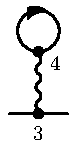
\includegraphics{sigma/sigma1a.pdf}
				\end{gathered}
			$}
	}
	+
	\raisebox{1.75ex}{
		\scalebox{0.75}{$
				\begin{gathered}
					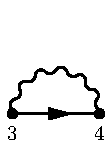
\includegraphics{sigma/sigma1b.pdf}
				\end{gathered}
			$}
	}
	+
	\hspace*{-1.25ex}
	\raisebox{1.75ex}{
		\scalebox{0.75}{$
				\begin{gathered}
					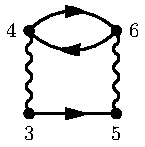
\includegraphics{sigma/sigma2a.pdf}
				\end{gathered}
			$}
	}
	\hspace*{-1.25ex}
	+
	\raisebox{1.75ex}{
		\scalebox{0.75}{$
				\begin{gathered}
					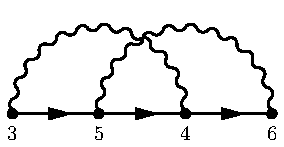
\includegraphics{sigma/sigma2b.pdf}
				\end{gathered}
			$}
	}
	+ \hspace*{1ex} \cdots
\end{equation*}
\end{document}
